\documentclass[10pt]{article}
\usepackage[margin=0.60in]{geometry}
\usepackage{amsmath,booktabs,enumitem,fancyhdr,graphicx,listings,tabularx,titlesec,xcolor}
\usepackage[hidelinks]{hyperref}
\graphicspath{{docs/lessons/assets/}{../assets/}}
\hypersetup{
 pdftitle={ADK Lesson 062: Thermal and Radiant Observations},
 pdfauthor={Kevin Shanahan},
 pdfsubject={Qualifying three independent copied thermal, categorical, and radiant evidence sources},
 pdflang={en-US}}
\pagestyle{fancy}\fancyhf{}
\lhead{\textsc{ADK Lesson 062}}\rhead{Thermal and Radiant Observations}
\cfoot{\thepage}\setlength{\headheight}{14pt}
\setlength{\parindent}{0pt}\setlength{\parskip}{3pt}
\setlist{nosep,leftmargin=1.45em}
\titleformat{\section}{\Large\bfseries}{\thesection}{0.5em}{}
\newcommand{\lessonbox}[1]{\begin{center}\fbox{\parbox{0.92\linewidth}{#1}}\end{center}}
\newcommand{\blankline}{\rule{0.76in}{0.4pt}}
\newcommand{\longblank}{\rule{1.35in}{0.4pt}}
\lstset{
 basicstyle=\ttfamily\footnotesize,
 columns=fullflexible,
 breaklines=true,
 frame=single,
 rulecolor=\color{black},
 showstringspaces=false}

\begin{document}
\small
\begin{center}
 {\Huge\bfseries Thermal and Radiant Observations}\\[3pt]
 {\Large Keep three copied sources distinct while finding hazards}\\[7pt]
 \fbox{\textbf{E0 SYNTHETIC REPLAY --- DO NOT WIRE OR ENERGIZE A SENSOR}}
\end{center}
\begin{tabularx}{\linewidth}{@{}>{\bfseries}l X >{\bfseries}l X@{}}
Lesson & 062 --- component & Time & 150--210 minutes\\
Prerequisites & status, supplied time, copied evidence & Board & compile-only Mega replay\\
Input & one three-source copied envelope & Observation & named memory result cell\\
\end{tabularx}

\lessonbox{\textbf{Responsibility.}
\texttt{ThermalRadiantObservationPolicy} preserves an already-converted
thermistor result, a distinct Digital Temperature threshold result, and a raw
radiant threshold result. It validates and ages each source independently,
then reports uncertainty, agreement, saturation, and hazard state. It owns no
sensor, pin, transport, conversion curve, clock, or stimulus.}

\section{Begin after acquisition, not before it}
The inventory names Thermistor, Digital Temperature, and Flame families, but
those labels are not electrical identities. Lesson 062 does not infer a
pinout, protocol, voltage, polarity, unit, or transfer curve from them.
Instead, synthetic producers copy three role-specific records across an E0
boundary. The policy evaluates those records without touching hardware.

\begin{center}
% ADK visual: pencil
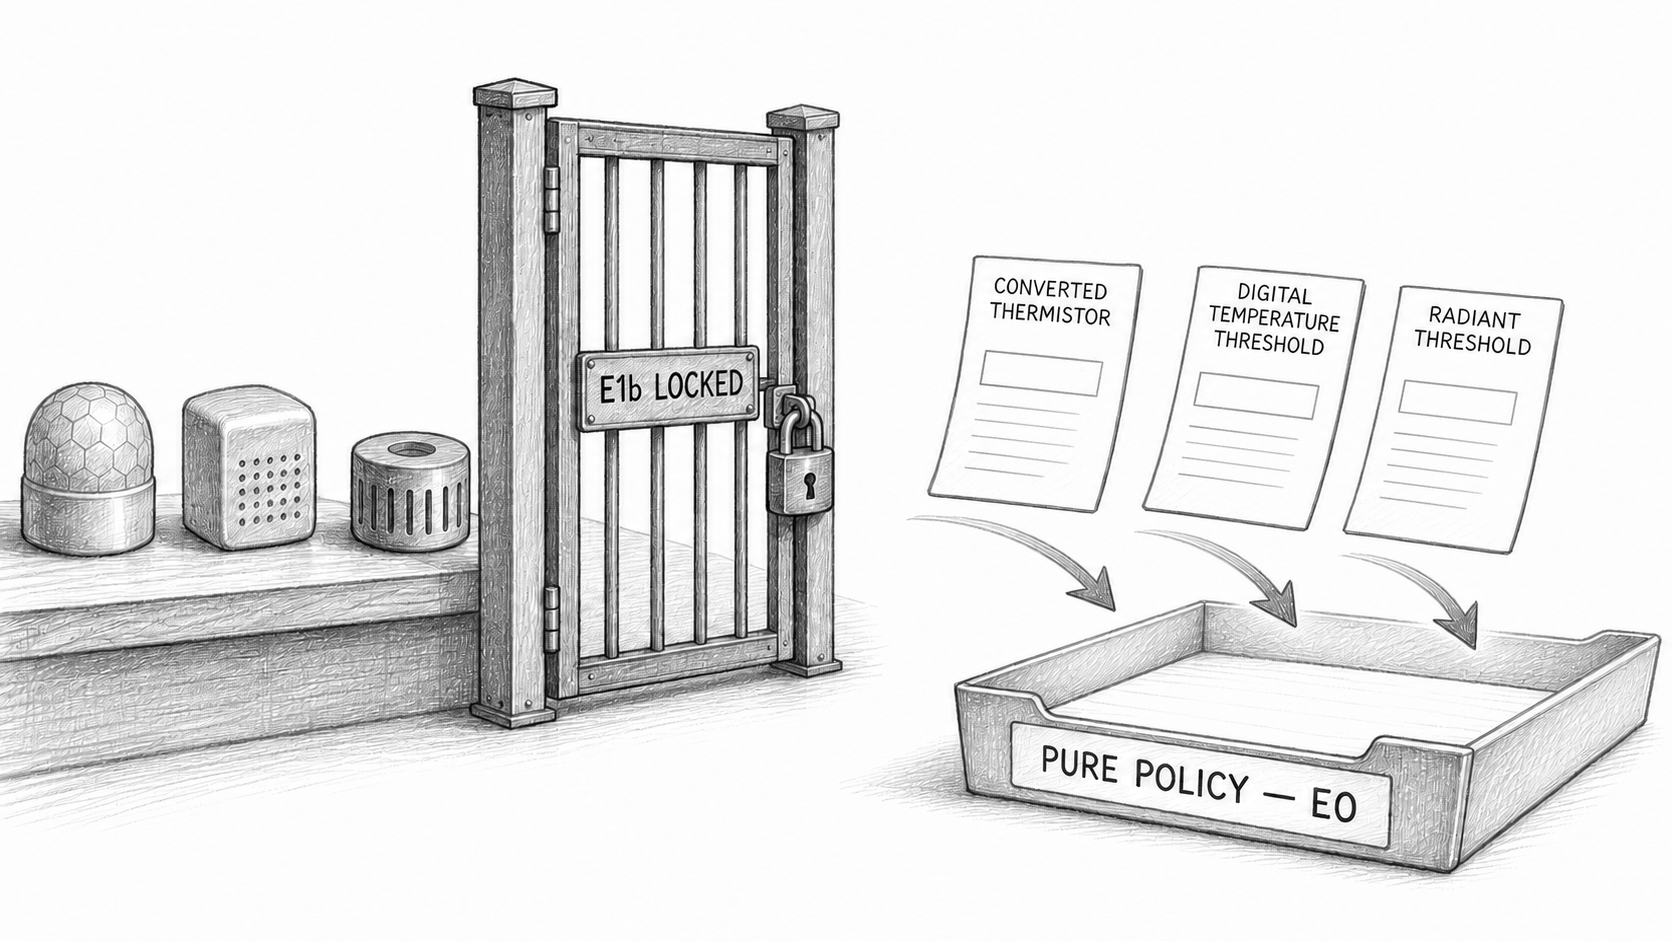
\includegraphics[width=0.95\linewidth,height=2.00in,keepaspectratio]
 {062-evidence-boundary-pencil.png}

\small\textit{Alternative text: a pencil drawing places three unidentified
physical specimens behind a locked E1b gate, while three copied cards---one
converted thermistor, one Digital Temperature threshold, and one radiant
threshold---enter a pure policy on the E0 side.}
\end{center}

\begin{tabularx}{\linewidth}{@{}X X@{}}
\toprule
E0 may establish & E0 does not establish\\
\midrule
deterministic interpretation of copied records & a module identity, adapter, or wiring diagram\\
role-specific provenance, sequence, and age & an ADC, GPIO, bus, timer, or supply claim\\
fixed uncertainty and threshold rules & a physical thermistor conversion curve\\
bounded radiant candidate state & flame, irradiance, temperature, or life-safety detection\\
\bottomrule
\end{tabularx}

There is no formal electrical schematic in this lesson. An authoritative
schematic requires exact specimens, primary evidence, measured rails and
currents, proved threshold polarity, and safe-state observations. Those E1b
requirements remain open.

\section{Copy three noninterchangeable records}
The thermistor producer supplies milli-degrees Celsius and an uncertainty.
The unidentified Digital Temperature producer supplies only a categorical
\texttt{Below} or \texttt{AtOrAbove} state plus a raw value. The radiant
producer supplies the same shape of categorical evidence, but its raw value
is unitless and its meaning remains radiant-threshold behavior.

\begin{center}
% ADK visual: pencil
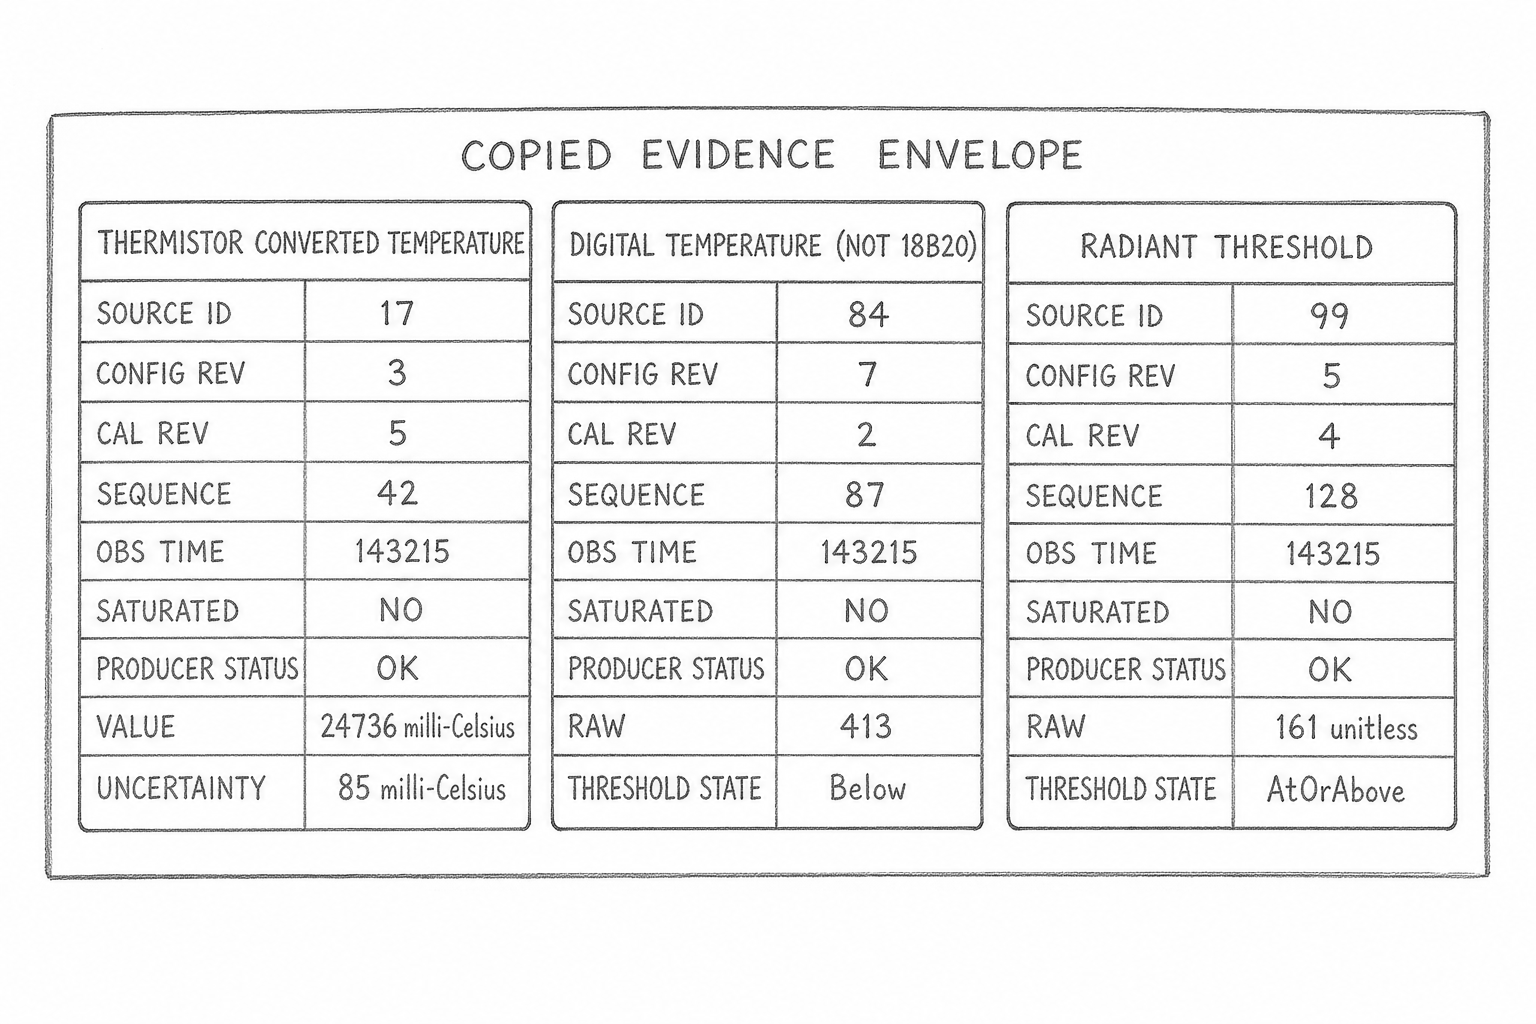
\includegraphics[width=0.96\linewidth,height=2.20in,keepaspectratio]
 {062-three-source-envelope-pencil.png}

\small\textit{Alternative text: three pencil-drawn cards share fields for
source, configuration, calibration, sequence, observation time, saturation,
and producer status; only the thermistor card has milli-Celsius and
uncertainty, while the other two have raw and threshold state.}
\end{center}

All three source IDs must be nonzero and mutually distinct. Each role retains
its own nonzero configuration and calibration revisions, nonzero sequence,
observation time, saturation flag, and producer status. The complete envelope
is copied; the policy retains no caller pointer. A marketplace family name is
not accepted as provenance.

\begin{tabularx}{\linewidth}{@{}l X@{}}
\toprule
Record & Honest E0 interpretation\\
\midrule
converted thermistor & temperature interval supplied by a synthetic producer\\
Digital Temperature & categorical threshold state; no protocol or temperature unit\\
radiant & unitless threshold activity; no flame or calibrated radiant unit\\
\bottomrule
\end{tabularx}

Explain why combining the two categorical cards into one generic ``hot
sensor'' would lose evidence: \longblank.

\section{Validate atomically before voting}
Configuration requires the warning temperature below the alarm temperature,
a wrap-safe maximum age, and nonzero wrap-safe radiant durations with
\(\text{pulse maximum}<\text{sustained minimum}\). Every accepted envelope
must preserve fixed role identities and revisions.

\begin{center}
% ADK visual: pencil
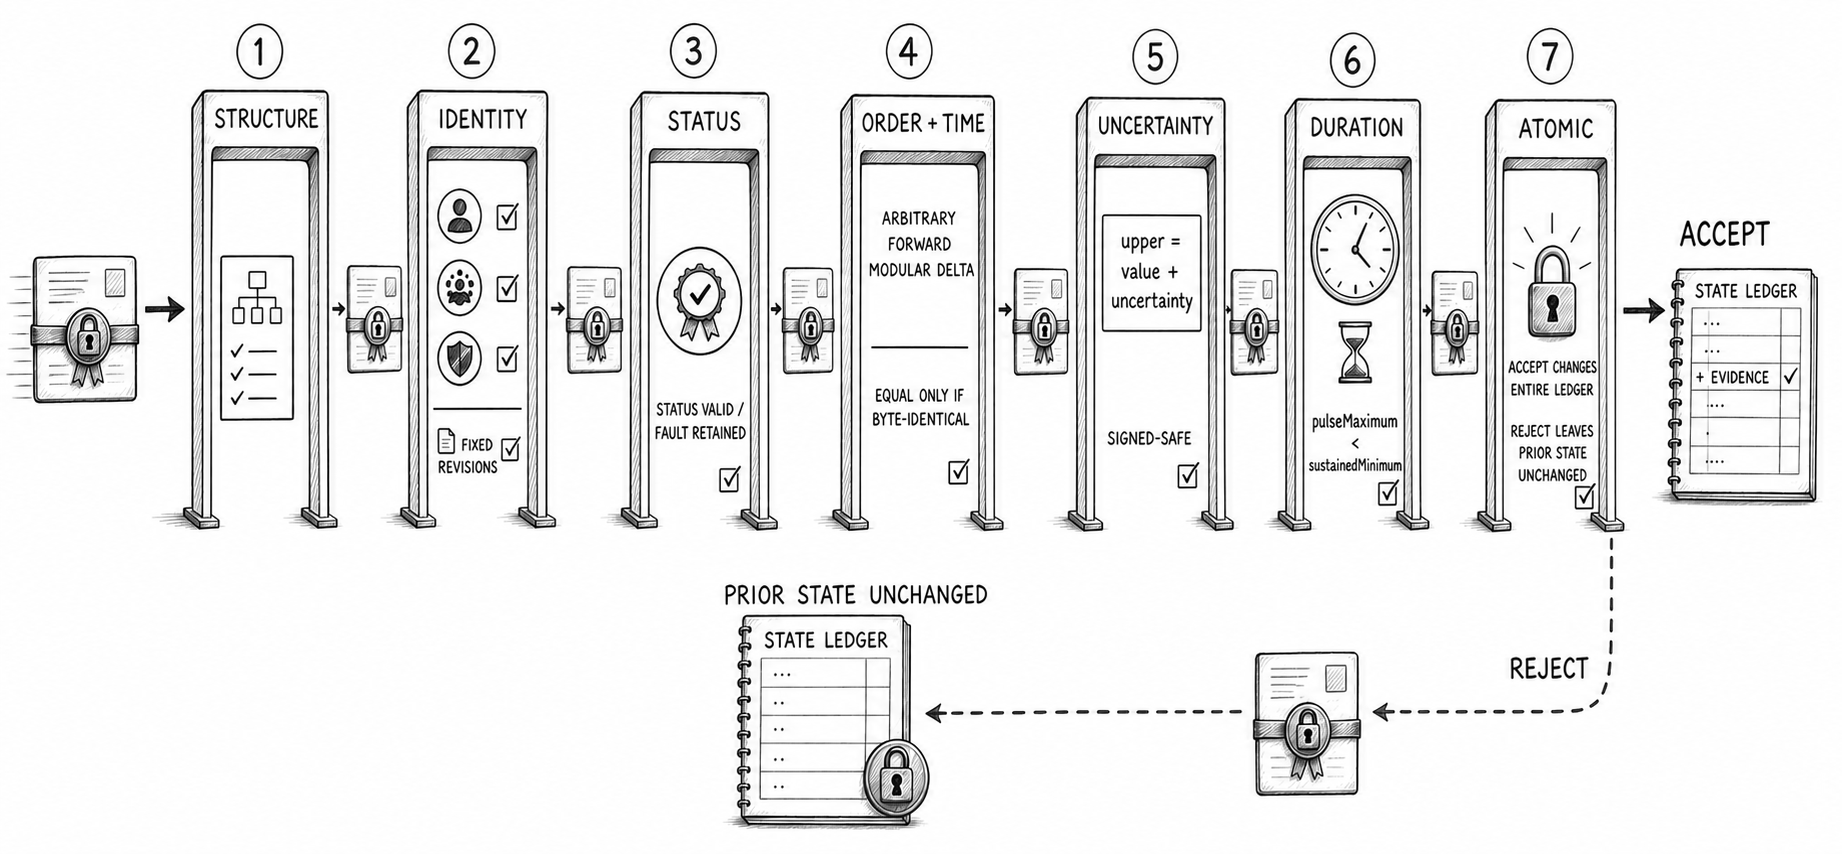
\includegraphics[width=0.95\linewidth,height=2.05in,keepaspectratio]
 {062-validation-gates-pencil.png}

\small\textit{Alternative text: a hand-drawn inspection line checks structure,
three distinct identities, revisions, producer status, independent sequence
and modular time, signed uncertainty arithmetic, and radiant duration
configuration before a sealed observation card may change.}
\end{center}

For each source, a byte-identical duplicate at equal sequence and time is
idempotent. A changed duplicate, regression, backward time, exact half-range
ambiguity, or identity/revision change rejects the whole update without
changing the last observation or radiant candidate. Sequence zero is invalid.
Once an accepted role reaches \texttt{UINT32\_MAX}, that role may remain
byte-identical while a companion role advances. Attempting to change the
exhausted role returns \texttt{CapacityExceeded}; only \texttt{reset()} begins
a new volatile sequence epoch.

Predict the result when the radiant record is malformed but the two thermal
records look normal: status \blankline; observation changes? \blankline.

\section{Classify a conservative temperature interval}
Only the thermistor path carries temperature units. Its supplied value \(v\)
and uncertainty \(u\) define explanatory bounds with widened signed
arithmetic:
\[
  \mathrm{lower}=v-u,\qquad \mathrm{upper}=v+u .
\]
The policy computes only the upper bound because it alone controls whether the
copied interval could reach a hazard. Tests use the lower endpoint as an
independent signed-extreme oracle:
\[
\begin{array}{ll}
 \mathrm{upper}<\mathrm{warning} & \texttt{Normal}\\
 \mathrm{upper}\geq\mathrm{alarm} & \texttt{Alarm}\\
 \mathrm{upper}\geq\mathrm{warning} & \texttt{Warning}.
\end{array}
\]

\begin{center}
% ADK visual: pencil
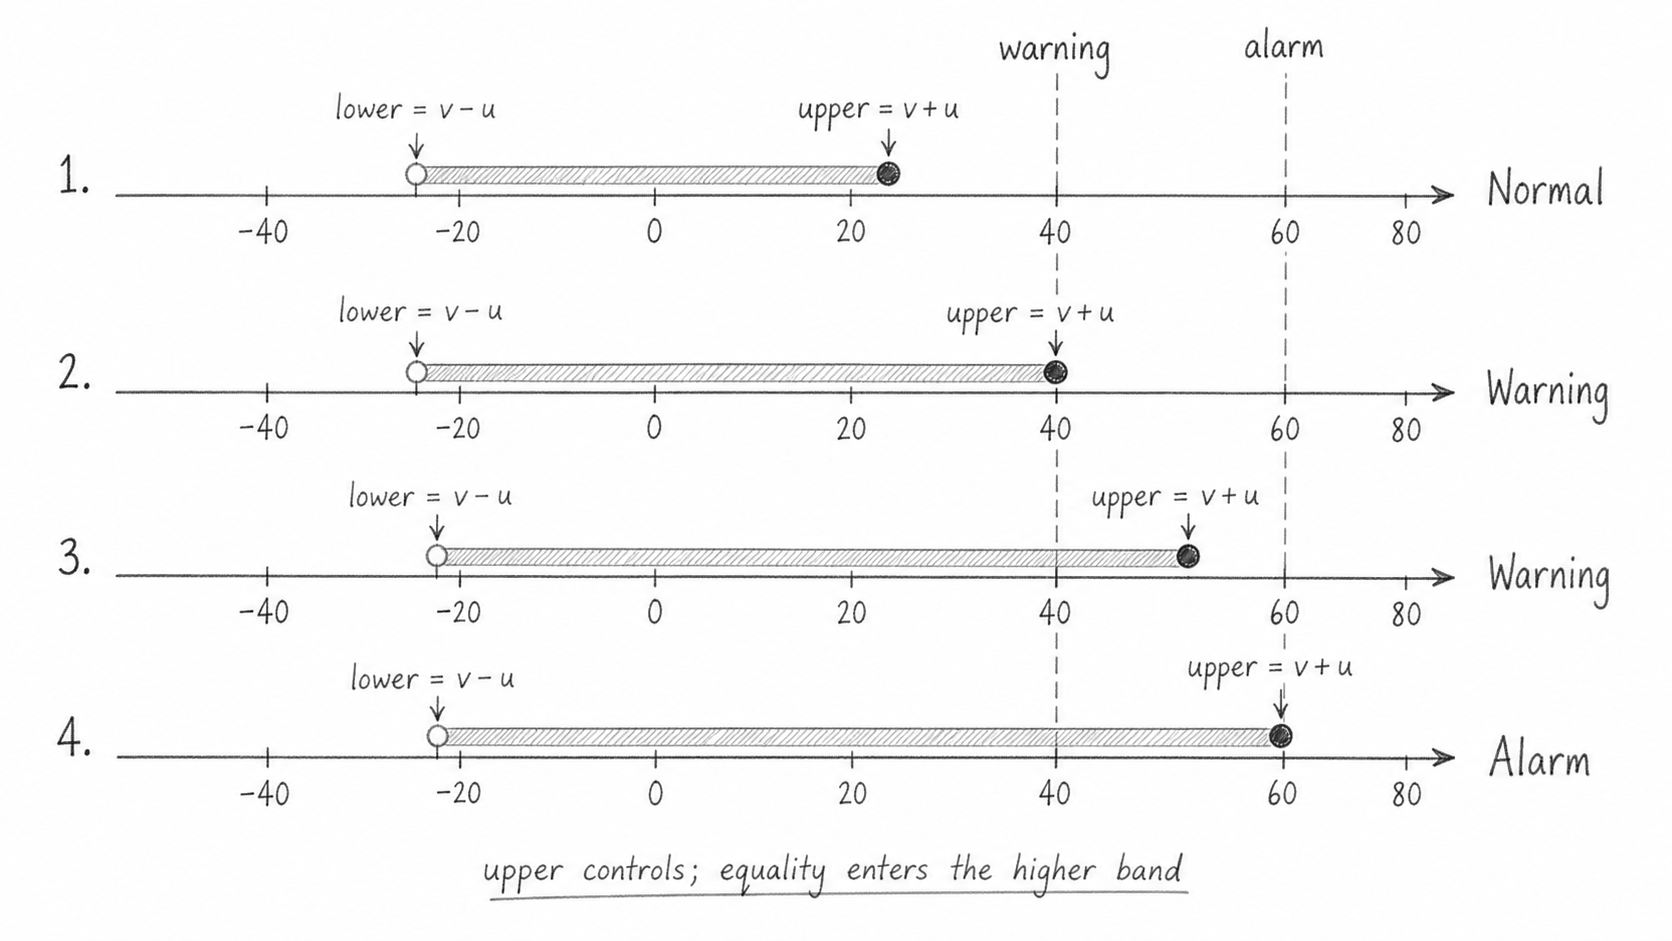
\includegraphics[width=0.95\linewidth,height=2.05in,keepaspectratio]
 {062-uncertainty-intervals-pencil.png}

\small\textit{Alternative text: pencil number lines show temperature
uncertainty intervals ending below warning, touching warning, lying between
warning and alarm, and touching alarm; equality moves conservatively into the
higher quality band.}
\end{center}

\begin{tabularx}{\linewidth}{@{}r r r l@{}}
\toprule
Value & Uncertainty & Upper bound & Thermistor result\\
\midrule
\(24{,}000\) & \(500\) & \(24{,}500\) & depends on configured warning\\
\(29{,}000\) & \(1{,}000\) & \(30{,}000\) & alarm if alarm is \(30{,}000\)\\
\(28{,}900\) & \(1{,}099\) & \(29{,}999\) & below that alarm boundary\\
\bottomrule
\end{tabularx}

With warning \(=25{,}000\) and alarm \(=30{,}000\), classify value
\(24{,}000\), uncertainty \(1{,}000\): \blankline. Then classify value
\(29{,}000\), uncertainty \(1{,}000\): \blankline.

\section{Preserve agreement without suppressing hazard}
The Digital Temperature mapping is fixed and categorical:
\texttt{AtOrAbove} means alarm and \texttt{Below} means normal. It supplies no
temperature value. A categorical alarm makes the combined thermal result
\texttt{Alarm}. A categorical normal paired with a thermistor warning or
alarm produces \texttt{Disagreement}; if the thermistor interval reaches
alarm, \texttt{thermalHazard} remains true.

\begin{center}
% ADK visual: pencil
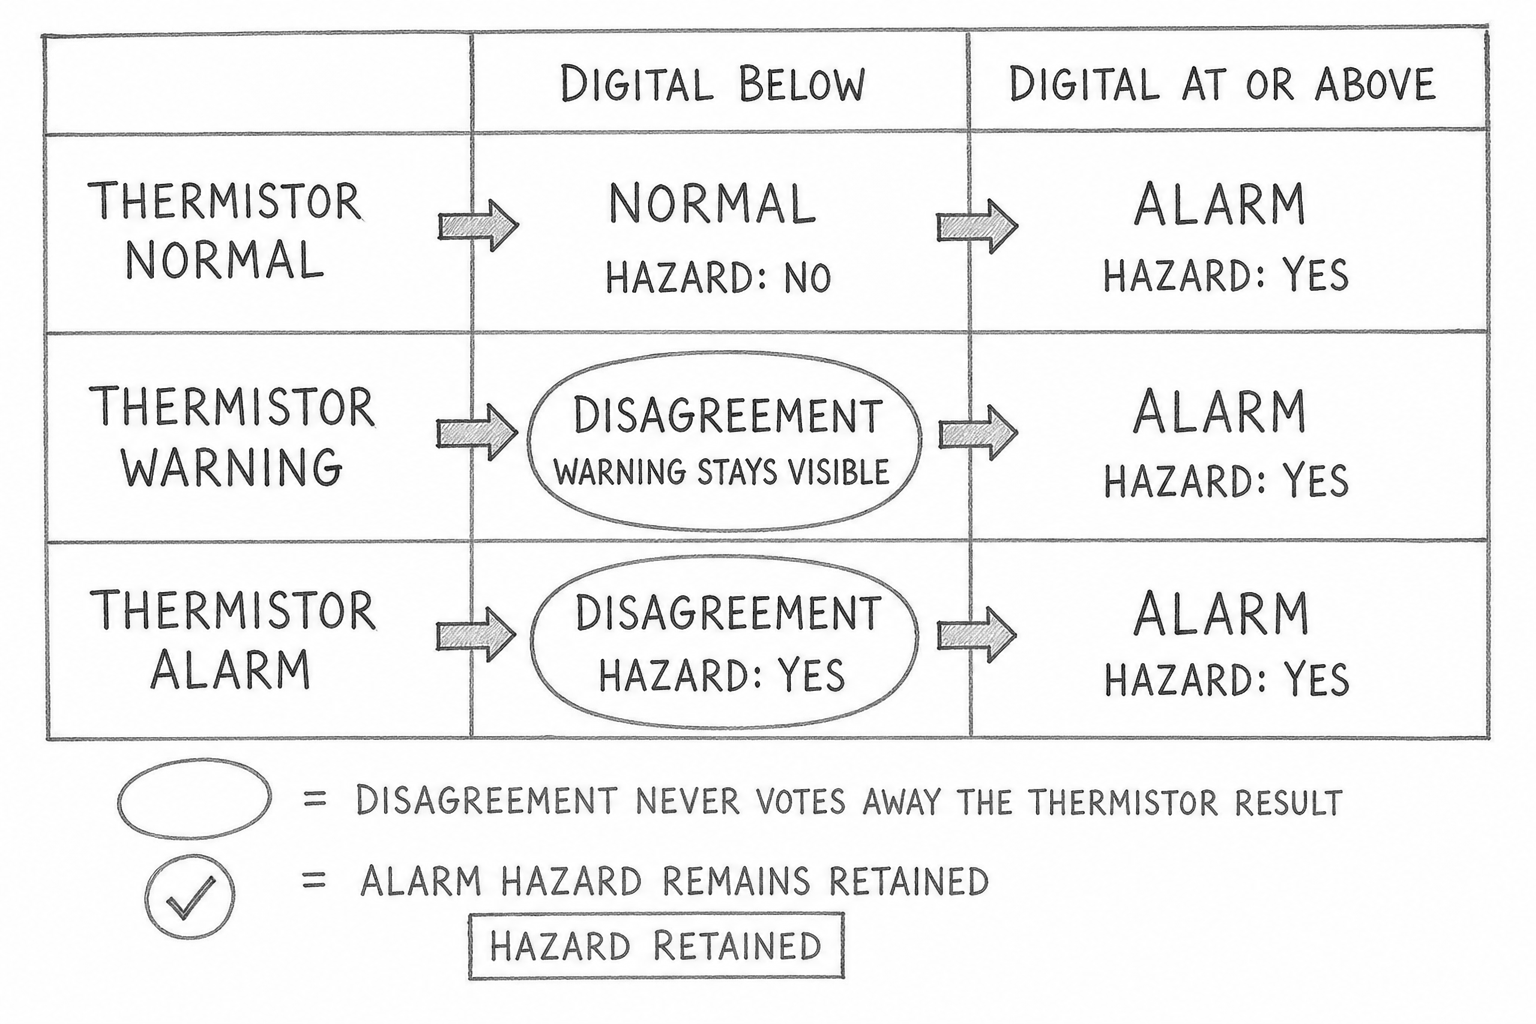
\includegraphics[width=0.96\linewidth,height=2.20in,keepaspectratio]
 {062-thermal-agreement-pencil.png}

\small\textit{Alternative text: a pencil matrix compares thermistor normal,
warning, and alarm rows with Digital Temperature below and at-or-above
columns; disagreement cells preserve the thermistor hazard flag instead of
voting it away.}
\end{center}

\begin{tabularx}{\linewidth}{@{}l l l X@{}}
\toprule
Thermistor & Digital state & Combined quality & Hazard rule\\
\midrule
normal & below & \texttt{Normal} & false\\
normal & at-or-above & \texttt{Alarm} & true\\
warning & below & \texttt{Disagreement} & warning remains visible\\
alarm & below & \texttt{Disagreement} & true; disagreement cannot suppress it\\
warning/alarm & at-or-above & \texttt{Alarm} & true\\
\bottomrule
\end{tabularx}

Stale, saturated, or producer-fault evidence never votes. Its side-specific
quality remains visible rather than being averaged into an attractive normal
result. Predict the safe interpretation of an alarm thermistor interval
paired with stale categorical evidence: \longblank.

When several copied producers report non-OK status together, the fixed status
precedence is thermistor, then Digital Temperature, then radiant. This selects
one deterministic reported status; it neither verifies a producer nor lets
any copied fault mutate policy state.

\section{Track a radiant candidate with supplied time}
Radiant threshold activity is temporal evidence, not temperature or flame
evidence. An inactive-to-active edge starts a candidate at its accepted
observation time. While active, elapsed time below the sustained minimum is
\texttt{AbruptChange}; equality and later are \texttt{Sustained}.

\begin{center}
% ADK visual: pencil
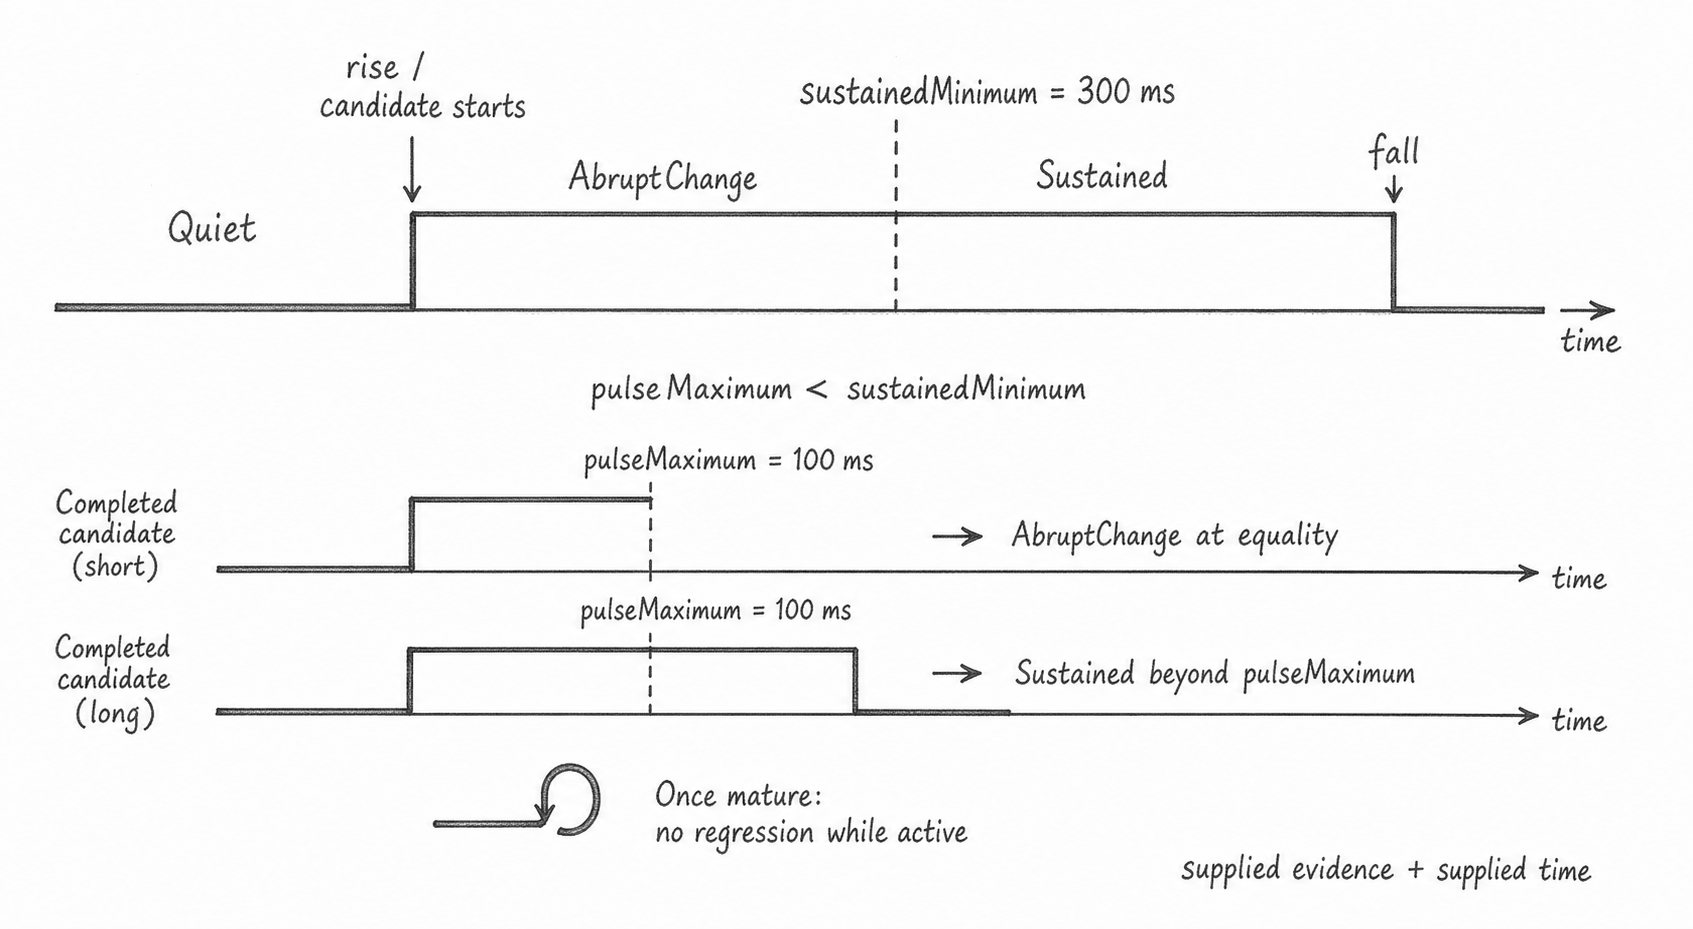
\includegraphics[width=0.95\linewidth,height=2.15in,keepaspectratio]
 {062-radiant-timeline-pencil.png}

\small\textit{Alternative text: a pencil timing strip shows inactive,
active-start, short abrupt activity, equality at the sustained threshold,
continued sustained activity, and an inactive edge; a second strip shows a
short completed pulse and a longer completed candidate.}
\end{center}

On an active-to-inactive edge, total elapsed time at or below the pulse
maximum reports \texttt{AbruptChange}; a longer completed candidate reports
\texttt{Sustained}. A byte-identical duplicate cannot extend duration.
Ambient saturation reports \texttt{SaturatedAmbient} and clears the
candidate, so later evidence must begin a new edge.

\begin{tabularx}{\linewidth}{@{}l l@{}}
\toprule
Boundary & Expected radiant quality\\
\midrule
active for sustained minimum minus one tick & \texttt{AbruptChange}\\
active for exactly sustained minimum & \texttt{Sustained}\\
inactive edge at exactly pulse maximum & \texttt{AbruptChange}\\
inactive edge one tick beyond pulse maximum & \texttt{Sustained}\\
ambient saturation & \texttt{SaturatedAmbient}; candidate cleared\\
\bottomrule
\end{tabularx}

If pulse maximum is 100 ms and sustained minimum is 300 ms, predict the result
of an inactive edge after 101 ms: \blankline. Explain why a duplicate at
250 ms cannot turn a 200 ms candidate into 250 ms of evidence: \longblank.

\section{Age each role independently}
\texttt{TimePoint now} is the only clock. The policy computes thermistor,
Digital Temperature, and radiant age separately with modular unsigned time.
Evidence exactly at maximum age is admitted; one tick older is stale. This
prevents a fresh source from laundering an old companion into a simultaneous
measurement.

\begin{center}
% ADK visual: pencil
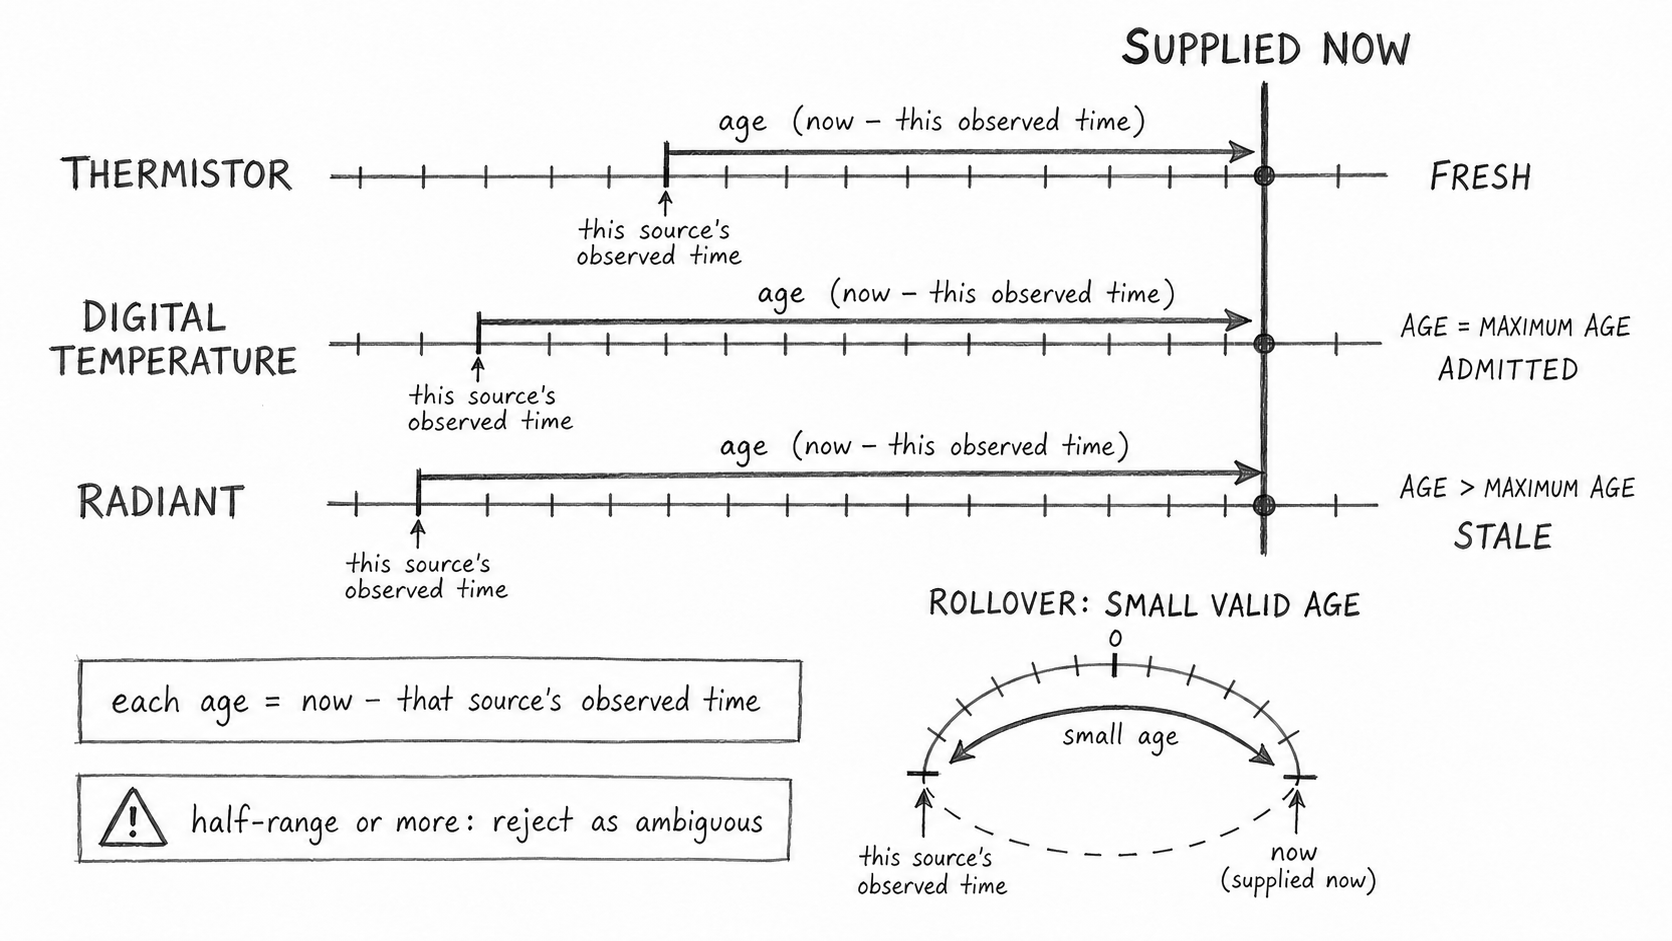
\includegraphics[width=0.94\linewidth,height=1.95in,keepaspectratio]
 {062-independent-ages-pencil.png}

\small\textit{Alternative text: three pencil clock tracks end at one supplied
now marker but begin at different observation times; one is fresh, one sits
on the inclusive maximum-age boundary, and one is stale, with a rollover arc
shown separately.}
\end{center}

Complete the diagnosis:
\begin{enumerate}
 \item thermistor age equals maximum age: \blankline;
 \item Digital Temperature age is one tick greater: \blankline;
 \item radiant time difference is exactly the modular half range:
       \blankline;
 \item thermistor crosses ordinary unsigned rollover with a small valid age:
       \blankline;
 \item reset then snapshot: quality \blankline, candidate active?
       \blankline.
\end{enumerate}

\section{Replay without stimulus or wiring}
The Mega example constructs synthetic envelopes, supplies time, updates the
policy, and copies snapshots into a named volatile result cell. It acquires
no ADC channel, pin, timer, bus, endpoint, display, or supply. Serial is not
the proof, and the compile-only replay makes no physical observation claim.

\begin{lstlisting}
ThermalRadiantObservationPolicy environment(config);
environment.initialize();

envelope.thermistor.sequence += 1U;
envelope.digitalTemperature.sequence += 1U;
envelope.radiant.sequence += 1U;
const Status updateStatus = environment.update(now, envelope);
const ThermalRadiantObservation result = environment.snapshot();
\end{lstlisting}

\begin{center}
% ADK visual: pencil
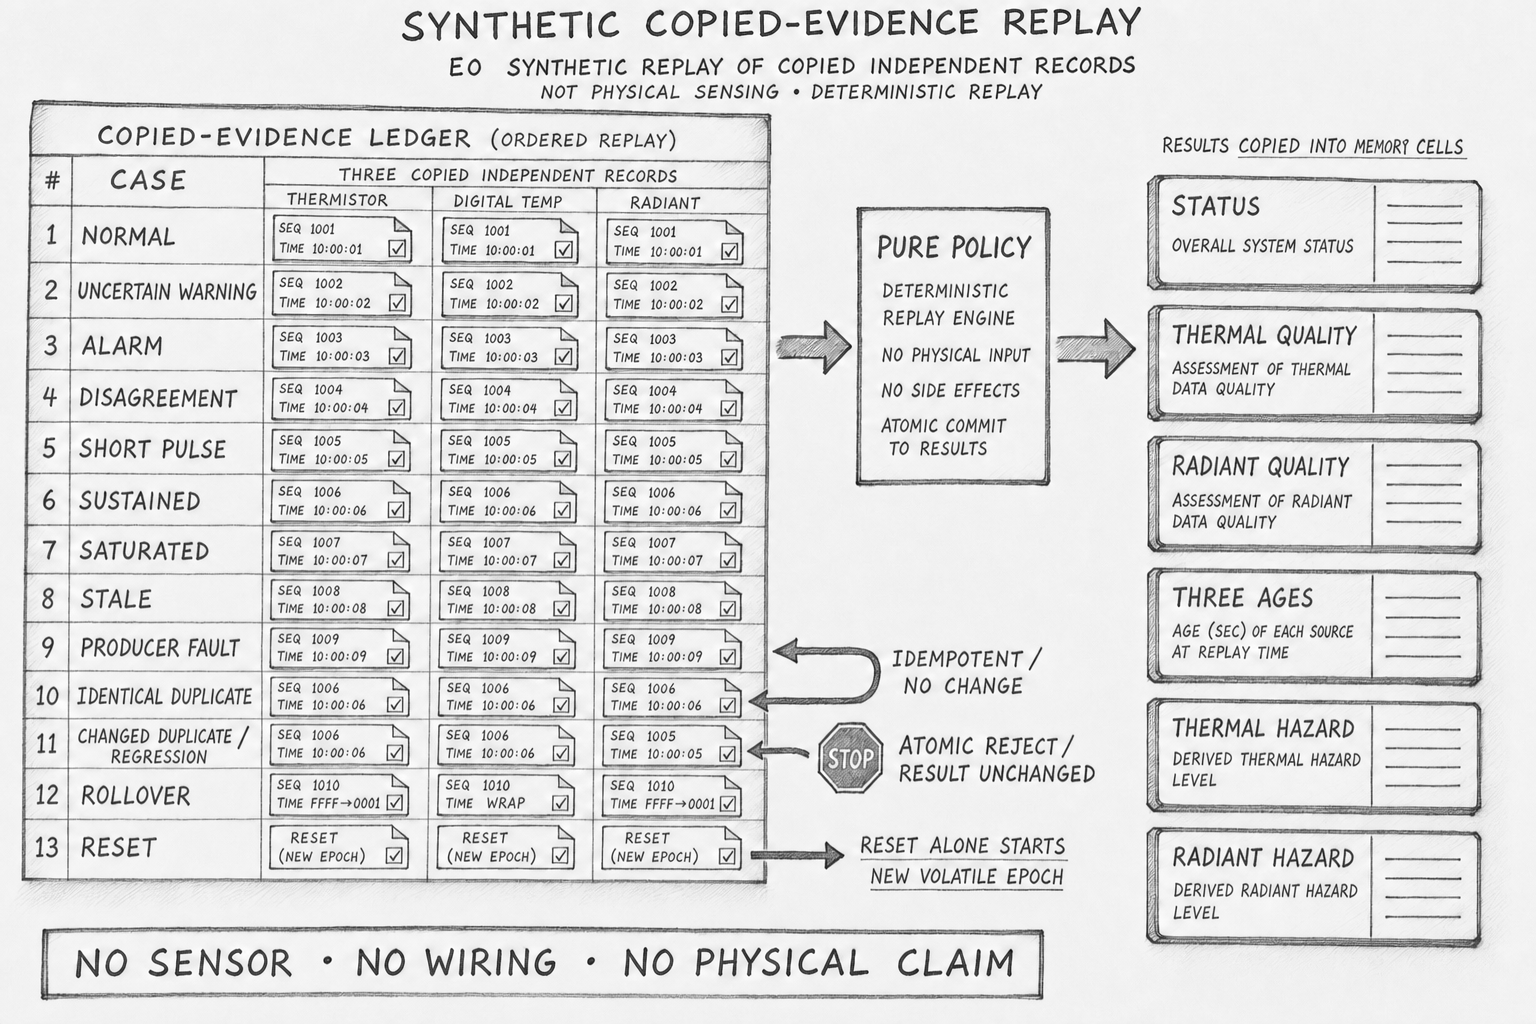
\includegraphics[width=0.95\linewidth,height=2.10in,keepaspectratio]
 {062-replay-ledger-pencil.png}

\small\textit{Alternative text: a pencil replay ledger feeds normal,
uncertain-warning, alarm, disagreement, short-pulse, sustained, saturated,
stale, producer-fault, duplicate, regression, rollover, and reset envelopes
into one policy and records status, both qualities, three ages, and two hazard
flags in named result cells.}
\end{center}

The deterministic proof must cover signed extrema; uncertainty immediately
below, at, and across both thermal thresholds; every categorical agreement
combination; radiant pulse and sustained neighbors; ambient saturation;
source collision; independent stale, future, and regressing records; changed
duplicates; producer faults; sequence exhaustion; rollover; reset; rejected
update atomicity; and byte-stable replay.

\section{Separate software evidence from open physical gates}
The canonical Mega replay measures 10,076 bytes of flash and 1,133 bytes of
static SRAM. The static-SRAM result is an independently accepted target miss
against 1,024 bytes and remains below the 1,536-byte hard limit. The exact
isolated no-LTO gate measures 5,156 bytes of flash, 279 bytes of static SRAM,
264 bytes of conservative synchronous stack, and a 112-byte policy object.
The caller retains 59 bytes of stack and a 76-byte observation, for 135
caller-owned bytes; 7,521 bytes of museum-monitor SRAM remain. These compiler
measurements are not runtime, electrical, optical, thermal, or physical
evidence.

\begin{tabularx}{\linewidth}{@{}l X X@{}}
\toprule
Gate & E0 pass evidence & Still open\\
\midrule
resource acquisition & zero hardware claims and compile-only replay & exact endpoints, rails, current, and ownership\\
safe state & reset and rejection clear or preserve bounded policy state & de-energized physical outputs and observation path\\
thermal & widened interval and agreement boundary tests & thermistor curve and Digital Temperature identity\\
radiant & pulse, sustained, saturation, and rollover traces & response, polarity, geometry, and harmless stimulus\\
replay & byte-stable named result cells & bench repeatability and physical acceptance\\
\bottomrule
\end{tabularx}

\lessonbox{\textbf{E1b remains open.}
Qualify the exact thermistor, the distinct Digital Temperature specimen, and
the radiant module independently before publishing an adapter, wiring,
physical units, or threshold polarity. Any radiant stimulus must be an owned,
documented harmless low-energy IR target/source pair or an owned TV remote
used only as a stimulus: attended, never aimed at eyes, active for at most
5 seconds, followed by at least 30 seconds inactive, and never replayed.
Lasers, flame, heaters, hot wire, combustible targets, ignition, continuous
or unattended exposure, and unknown targets are excluded.}

E1b also requires a non-Serial observation path plus separate proof of
resource acquisition and physical safe state. Lesson 062 contains no powered
acceptance record and makes no life-safety, fire-detection, preservation, or
absence-of-hazard claim.

\section{Completion record}
\begin{tabularx}{\linewidth}{@{}X X@{}}
\toprule
Check & Result or evidence\\
\midrule
Three distinct roles, identities, revisions, and copied fields & \\
\addlinespace[1.2em]
Signed widened uncertainty and both threshold neighbors & \\
\addlinespace[1.2em]
Every thermal/categorical agreement and hazard result & \\
\addlinespace[1.2em]
Radiant pulse, sustained, saturation, and candidate reset & \\
\addlinespace[1.2em]
Independent age, duplicate, regression, exhaustion, and rollover & \\
\addlinespace[1.2em]
Atomic rejection, reset, replay, and named result cells & \\
\addlinespace[1.2em]
Zero-hardware E0 boundary and all open E1b work & \\
\addlinespace[1.2em]
\bottomrule
\end{tabularx}

\begin{center}
\fbox{\parbox{0.90\linewidth}{
\textbf{Completion statement:} I can distinguish converted temperature from
categorical threshold and radiant evidence, apply conservative uncertainty
and disagreement rules, reproduce every radiant timing boundary, and name the
electrical and physical claims that remain open.

\vspace{0.10in}
Learner: \longblank\quad Reviewer: \longblank\quad Date: \blankline
}}
\end{center}

This print edition is untagged. Its text is searchable and copyable, and the
HTML lesson provides the hardware-independent alternative. No PDF/UA, WCAG,
or other PDF accessibility-conformance claim is made.

\end{document}
